\documentclass[10pt]{article}

\usepackage[margin=1in]{geometry}
\usepackage{amsmath,amssymb}
\usepackage{booktabs}
\usepackage{graphicx}
\usepackage{float}
\usepackage{microtype}
\usepackage[numbers,sort&compress]{natbib}
\usepackage[hidelinks]{hyperref}
\usepackage{enumitem}
\usepackage{xcolor}
\usepackage{tikz}
\usetikzlibrary{arrows.meta,positioning,shapes.geometric}

\graphicspath{{figures_pdf/}{figures/}}
\setlist[itemize]{leftmargin=1.5em}
\setlist[enumerate]{leftmargin=1.5em}

\title{Inference Acceleration as Closed-Loop Perturbation:\\
Closed-Loop Sensitivity-Guided Tactic Search for VLA Policies}
\author{patrick.zhang\\\href{mailto:patrick.zhang5233@gmail.com}{\texttt{patrick.zhang5233@gmail.com}}}
\date{}

\newcommand{\fp}{\mathrm{fp16}}
\newcommand{\dpi}{d_{\pi_\theta}}
\newcommand{\da}{d_{\pi_\varphi}}
\newcounter{clsgalgorithm}
\renewcommand{\theclsgalgorithm}{\arabic{clsgalgorithm}}

\begin{document}
\maketitle

\begin{abstract}
Inference acceleration for vision-language-action (VLA) policies is usually framed as a local systems problem: quantize weights, compile graphs, fuse kernels, or replay static execution paths, then check numerical drift and serving latency. This framing misses the central difficulty for robot policies. The accelerated model is not only an approximator of a fixed function; it is a controller inside a feedback loop. A small implementation perturbation can change contact timing, future observations, receding-horizon replanning, and ultimately whether a rollout crosses a thresholded success margin.

We formulate post-training VLA acceleration as a closed-loop policy perturbation problem and propose Closed-Loop Sensitivity-Guided Tactic Search (CLSG-TS), a practical procedure for selecting acceleration tactics under rollout budget. The method first uses cheap static and open-loop filters to prune candidate tactics, then evaluates the surviving candidates on matched fragile rollouts, estimates closed-loop risk from paired repairs/regressions and first-divergence diagnostics, and finally selects a behavior-first, speed-constrained, or routed deployment point on a held-out speed--risk frontier.

This framework yields five claims that organize the study: implementation error is filtered by closed-loop sensitivity; rollout flips are margin-crossing events; fixed-distribution validation is insufficient without state-distribution control; sensitivity is anisotropic across action channels, rollout phases, and model boundaries; and acceleration is best understood as constrained exploration of nearby policy implementations rather than imitation of one FP16 point. We test these claims on GR00T policies in LIBERO-10 using \texttt{torch.compile} action-head acceleration, eager-island and duration fallback tactics, controlled action perturbations, first-divergence traces, matched repair/regression accounting, and held-out tactic routing.

The empirical picture is non-monotonic. Speed-only action-head compilation gives a 2.23$\times$ median server-latency speedup on a 33-case GR00T N1.5 probe, yet reduces success from 19/33 to 16/33. CLSG-TS recovers behavior without simply reverting to FP16: an early-block eager island reaches 18/33 at 2.31$\times$ speedup, and a fine duration probe finds that protecting policy steps 0--120 restores 19/33 at 69.66 ms versus 156.22 ms for FP16. Held-out validation then changes the conclusion from ``choose the local winner'' to ``choose a point on a speed--risk frontier.'' Across two N1.5 30-case folds, speed-only execution is fastest but has 7 paired regressions; the 0--120 duration tactic and a combined early-block plus 0--120 tactic both reach 47/60 pooled success with different speed--risk trade-offs. A GR00T N1.7 held-out check shows the same structure and motivates task-conditioned tactic routing as a high-speed but still validation-dependent option.

We do not claim universal superiority of any single backend or tactic. The contribution is a method for VLA acceleration under closed-loop risk: estimate which perturbations are sensitive, then select compilation, fallback, kernel, quantization, or routing tactics by matched rollout repair/regression and latency rather than by one-step drift or a single probe winner.
\end{abstract}

\section{Introduction}

Large vision-language-action models are increasingly used as generalist robot policies. They map visual observations and language instructions into action chunks, often through diffusion-style denoising or transformer action heads. As these models grow, inference acceleration becomes unavoidable: deployment systems will quantize weights, compile graphs, fuse kernels, cache repeated structure, replay static CUDA graphs, or mix high- and low-precision execution. The usual evaluation asks whether the accelerated implementation is numerically close to the reference policy and faster to serve.

For closed-loop robot policies, numerical closeness is not the whole problem. An action difference at time $t$ changes the next observation. The next action is then produced on a state that may not have been visited by the original FP16 policy. In manipulation, this feedback loop can change contact timing, grasp stability, object pose, or whether the terminal state crosses a binary success predicate. A tiny implementation difference can be absorbed in one phase, amplified near a contact boundary, or even repair a failure by nudging the rollout into a different trajectory basin.

This paper studies the following question:
\begin{quote}
How should VLA inference acceleration be designed and evaluated when the accelerated implementation is part of a closed-loop control system?
\end{quote}

Our answer is that post-training acceleration should be treated as a structured policy perturbation. Quantization, graph compilation, eager islands, and kernel replacement are different implementation maps from a reference policy to a constrained, faster policy. The relevant object is not only the one-step action drift on fixed observations, but also how the implementation redistributes success and failure over matched closed-loop rollouts. This changes the goal from finding a single numerically closest implementation to mapping a speed--behavior design space.

We organize the paper around five claims:
\begin{enumerate}
    \item \textbf{Closed-loop filtering:} acceleration-induced action error matters through dynamics, policy feedback, and future closed-loop gain, not only through its norm.
    \item \textbf{Margin and basin sensitivity:} rollout flips occur when perturbations cross task success margins or trajectory-basin boundaries.
    \item \textbf{Open-loop insufficiency:} fixed-distribution action drift cannot predict behavior under the accelerated policy's own induced state distribution.
    \item \textbf{Anisotropic sensitivity:} action channels, rollout durations, and model-layer boundaries are not equally sensitive.
    \item \textbf{Solution-space exploration:} acceleration can create repairs and regressions, so the useful target is not blind FP16 imitation but sensitivity-guided search for faster implementations with better paired repair/regression trade-offs.
\end{enumerate}

The paper follows a single arc. We first derive why local implementation error must be weighted by closed-loop dynamics and task margins. We then identify where perturbations matter most across action dimensions, rollout phases, and execution boundaries. Finally, we turn those sensitivity maps into CLSG-TS and validate the resulting speed--risk frontier on held-out folds and a newer checkpoint. Our contributions are:
\begin{enumerate}
    \item We formulate VLA inference acceleration as a closed-loop policy perturbation problem and derive local propagation, margin-crossing, and distribution-shift expressions that explain why local drift is not sufficient.
    \item We propose CLSG-TS, a rollout-budget-aware tactic-search workflow that combines cheap filters, fragile matched probes, first-divergence diagnostics, paired repair/regression accounting, and held-out speed--risk selection.
    \item We show that action channels, rollout phases, and action-head execution boundaries have strongly anisotropic closed-loop sensitivity, so equal-size implementation perturbations can have different behavioral effects.
    \item We show that speed-only action-head compilation can be fast but behaviorally unsafe, and that sensitivity-guided eager islands and duration fallbacks can recover behavior while preserving much of the latency gain.
    \item We show that a strong local tactic, policy steps 0--120, is not universal: multi-fold validation and an N1.7 held-out check change the conclusion from selecting one fixed winner to selecting behavior-first, speed-constrained, or routed tactics by worst-fold success, paired regressions, and latency.
\end{enumerate}

\paragraph{From point solution to design-space map.}
The contribution is not a single deployment backend. We use compilation, fallback, and routing probes to expose the geometry of the problem: which perturbations are absorbed, which are amplified, which rollouts are repaired or regressed, and which dimensions, phases, or modules should be protected. The intended output is therefore a map of the acceleration design space and a tactic-selection procedure, not only a point estimate for one checkpoint.

\paragraph{Model-class interpretation.}
Our findings are not tied to a specific checkpoint-level failure pattern. They suggest a model-class behavior: for DiT-style VLA or world-action models, small acceleration-induced implementation perturbations are filtered through closed-loop sensitivity, task margins, and trajectory basins. Larger or newer GR00T-style variants, as well as related action-diffusion policies, should therefore be evaluated by re-estimating their sensitivity maps rather than assuming uniform acceleration tolerance across dimensions, time, or layers.

\paragraph{Scope of claims.}
This paper should be read as a behavior-level modeling and tactic-selection study, not as a new compiler or production deployment benchmark. The acceleration track uses prototype action-head execution boundaries and fallback windows. We do not claim final memory, energy, or production backend performance. We also do not treat small aggregate success-rate gaps as policy dominance. The main claim is methodological: VLA acceleration should be evaluated and designed as sensitivity-weighted closed-loop perturbation, using matched rollouts and paired repair/regression analysis rather than only average open-loop action error or raw serving latency.

\paragraph{Experimental roadmap.}
The experiments are intentionally staged so that each stage answers the question raised by the previous one. First, controlled action perturbations and layer/boundary probes identify sensitive directions, rollout windows, and execution boundaries. Second, mixed eager/compiled acceleration policies test whether those maps can guide a faster implementation. Third, held-out folds and the N1.7 check show why the final object should be a robust tactic-selection protocol rather than a single fixed window.

\section{Related Work}

\paragraph{Vision-language-action policies.}
Recent robot policies increasingly combine large-scale visual, language, and action modeling. RT-1 introduced a scalable transformer policy trained on diverse real-robot data~\citep{rt1}. RT-2 framed robotic actions as tokens inside a vision-language-action model and showed transfer from web-scale vision-language training to control~\citep{rt2}. OpenVLA made this direction more accessible by releasing a 7B-parameter open-source VLA trained on large robot demonstration mixtures, and also noted practical interest in efficient fine-tuning and quantized serving~\citep{openvla}. GR00T N1 uses a dual-system VLA architecture where a vision-language module conditions a diffusion transformer action module~\citep{grootn1}. Diffusion Policy and related action-diffusion methods model robot behavior as conditional denoising, often with receding-horizon control~\citep{diffusionpolicy}. Our work focuses on the evaluation problem that appears when such policies are compressed or accelerated after training.

\paragraph{Inference acceleration for closed-loop policies.}
Deployment acceleration can come from low-precision arithmetic, graph compilation, operator fusion, CUDA graph replay, caching, or custom kernels. In open-loop perception or language tasks, small numerical differences are usually judged by output agreement and throughput. In VLA policies, the accelerated implementation chooses actions that alter future observations. This makes acceleration a behavioral question as well as a systems question: a faster implementation is useful only if its closed-loop policy perturbation stays within acceptable task margins.

\paragraph{Post-training acceleration and quantization.}
Post-training acceleration includes graph compilation, operator fusion, kernel replacement, mixed precision, and low-bit quantization. PTQ methods for large transformers often target memory and latency while preserving model quality. LLM.int8() handles transformer outliers through mixed-precision decomposition~\citep{llmint8}; GPTQ uses approximate second-order information for one-shot low-bit weight quantization~\citep{gptq}; SmoothQuant migrates quantization difficulty from activations to weights through an equivalent smoothing transform~\citep{smoothquant}; and AWQ uses activation statistics to protect salient weight channels~\citep{awq}. QuantVLA is the most direct prior work on PTQ for VLA systems, proposing scale-calibrated selective quantization, attention temperature matching, and output head balancing~\citep{quantvla}. These systems motivate our setting, but our contribution is not another quantizer. We study the closed-loop tactic-selection problem that arises for any post-training implementation change, including compilation, fallback routing, custom kernels, and future low-precision backends.

\paragraph{Sequential prediction and distribution shift.}
The gap between offline error and closed-loop behavior is a classic issue in imitation learning and sequential prediction. DAgger formalizes the problem that future observations depend on previous actions, so policies trained or evaluated only under a fixed data distribution can suffer from compounding errors~\citep{dagger}. VLA acceleration creates a related but distinct problem: the policy is already trained, but a post-training implementation change perturbs its action outputs and therefore perturbs the state distribution it induces. This makes paired rollout analysis a natural complement to fixed-distribution action-drift checks.

\paragraph{Feedback control perspective.}
Classical feedback control emphasizes that closed-loop behavior is determined by the interaction between controller perturbations, plant dynamics, and feedback gain~\citep{astrom2008feedback}. We use this lens to interpret inference acceleration not as a static approximation problem, but as a bounded policy perturbation whose effect depends on local closed-loop sensitivity and task margins.

\section{Inference Acceleration as Policy Perturbation}

Let $\pi_\theta(a \mid s,l)$ denote a reference FP16 VLA policy conditioned on state observation $s$ and language instruction $l$. A post-training acceleration transform constructs an implemented policy
\begin{equation}
    \varphi = \mathcal{A}(\theta; C, S), \qquad \pi_\varphi = \pi_{\varphi},
\end{equation}
where $\mathcal{A}$ may represent graph compilation, mixed-precision partitioning, kernel replacement, graph replay, fallback routing, or quantization; $C$ denotes calibration or profiling data when applicable; and $S$ denotes systems choices such as compilation boundaries, fallback windows, tactic selectors, or shape buckets. Even without gradient updates, this is not a neutral storage transform: it changes the implemented function.

Offline action drift measures a local difference such as
\begin{equation}
    e(s) = \left\| \pi_\varphi(s,l) - \pi_\theta(s,l) \right\|
\end{equation}
on observations sampled from some dataset or reference rollout distribution. Closed-loop performance depends on the state distributions induced by the two policies, $\dpi$ and $\da$.

For a local transition model,
\begin{equation}
    s_{t+1}=f(s_t,a_t), \qquad a_t=\pi(s_t),
\end{equation}
a first-order error expansion gives
\begin{equation}
    \delta s_{t+1} \approx J_s \delta s_t + J_a \delta a_t,
    \qquad
    \delta a_t = \pi_\varphi(s_t)-\pi_\theta(s_t).
\end{equation}
Even if $\delta a_t$ is small on the reference rollout distribution, the accumulated $\delta s_t$ can move the accelerated policy into states where the original local error estimate no longer applies.

This is why manipulation success is not a smooth function of single-step action MSE. A rollout can flip because of a small action perturbation if that perturbation changes whether the gripper reaches the object before closing, whether a placed object crosses a success-region boundary, whether an object contact produces a different pose, or whether a receding-horizon action chunk enters a different trajectory basin. In this view, acceleration is closer to post-training policy editing than to passive systems optimization.

\begin{figure}[H]
    \centering
    \resizebox{0.96\linewidth}{!}{%
    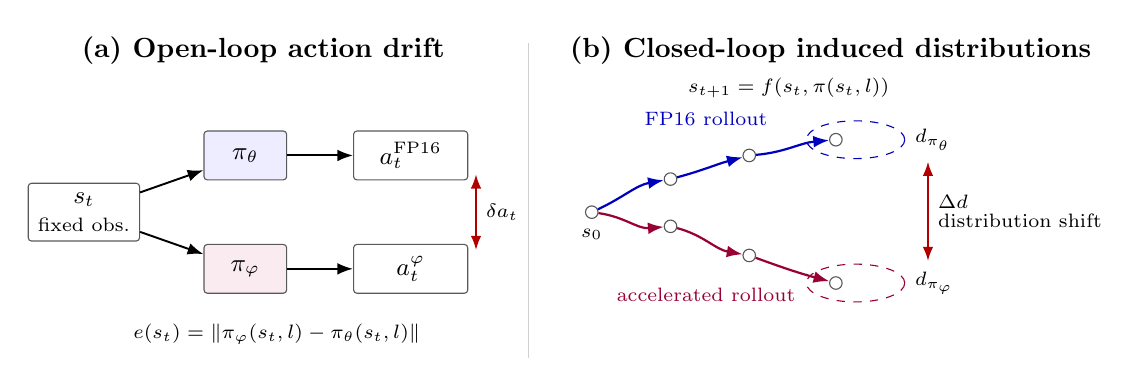
\begin{tikzpicture}[
        font=\small,
        box/.style={draw=black!65, rounded corners=1.2pt, align=center, inner sep=3.5pt, minimum height=0.62cm},
        policy/.style={box, fill=blue!7},
        implpolicy/.style={box, fill=purple!8},
        state/.style={circle, draw=black!65, fill=white, inner sep=1.6pt},
        arr/.style={-{Latex[length=2mm]}, line width=0.7pt},
        darr/.style={{Latex[length=1.8mm]}-{Latex[length=1.8mm]}, line width=0.65pt},
        trajfp/.style={-{Latex[length=2mm]}, line width=0.8pt, draw=blue!75!black},
        trajq/.style={-{Latex[length=2mm]}, line width=0.8pt, draw=purple!80!black}
    ]
        \node[anchor=west, font=\bfseries] at (-0.15, 2.05) {(a) Open-loop action drift};
        \node[box, minimum width=1.35cm] (obs) at (0, 0) {$s_t$\\[-1pt]\scriptsize fixed obs.};
        \node[policy, minimum width=1.05cm] (pifp) at (2.05, 0.72) {$\pi_\theta$};
        \node[implpolicy, minimum width=1.05cm] (piq) at (2.05, -0.72) {$\pi_\varphi$};
        \node[box, minimum width=1.45cm] (afp) at (4.15, 0.72) {$a_t^{\mathrm{FP16}}$};
        \node[box, minimum width=1.45cm] (aq) at (4.15, -0.72) {$a_t^\varphi$};
        \draw[arr] (obs) -- (pifp);
        \draw[arr] (obs) -- (piq);
        \draw[arr] (pifp) -- (afp);
        \draw[arr] (piq) -- (aq);
        \draw[darr, draw=red!70!black] (4.98, 0.48) -- node[right, font=\scriptsize] {$\delta a_t$} (4.98, -0.48);
        \node[align=center, font=\scriptsize] at (2.45, -1.55)
            {$e(s_t)=\|\pi_\varphi(s_t,l)-\pi_\theta(s_t,l)\|$};

        \draw[black!18, line width=0.5pt] (5.65, -1.85) -- (5.65, 2.15);

        \node[anchor=west, font=\bfseries] at (6.05, 2.05) {(b) Closed-loop induced distributions};
        \node[font=\scriptsize, align=center] at (8.95, 1.58)
            {$s_{t+1}=f(s_t,\pi(s_t,l))$};

        \node[state, label=below:{\scriptsize $s_0$}] (s0) at (6.45, 0) {};
        \node[state] (f1) at (7.45, 0.42) {};
        \node[state] (f2) at (8.45, 0.72) {};
        \node[state] (f3) at (9.55, 0.92) {};
        \node[state] (q1) at (7.45, -0.18) {};
        \node[state] (q2) at (8.45, -0.55) {};
        \node[state] (q3) at (9.55, -0.9) {};

        \draw[trajfp] (s0) to[out=25,in=190] (f1);
        \draw[trajfp] (f1) to[out=15,in=195] (f2);
        \draw[trajfp] (f2) to[out=5,in=185] (f3);
        \draw[trajq] (s0) to[out=-8,in=185] (q1);
        \draw[trajq] (q1) to[out=-15,in=170] (q2);
        \draw[trajq] (q2) to[out=-20,in=165] (q3);

        \node[draw=blue!75!black, dashed, ellipse, minimum width=1.25cm, minimum height=0.48cm,
              label=right:{\scriptsize $d_{\pi_\theta}$}] at (9.8, 0.92) {};
        \node[draw=purple!80!black, dashed, ellipse, minimum width=1.25cm, minimum height=0.48cm,
              label=right:{\scriptsize $d_{\pi_\varphi}$}] at (9.8, -0.9) {};
        \draw[darr, draw=red!70!black] (10.72, 0.64) --
            node[right, font=\scriptsize, align=left] {$\Delta d$\\[-1pt]\scriptsize distribution shift}
            (10.72, -0.62);

        \node[font=\scriptsize, text=blue!75!black] at (7.9, 1.18) {FP16 rollout};
        \node[font=\scriptsize, text=purple!80!black] at (7.9, -1.05) {accelerated rollout};
    \end{tikzpicture}}
    \caption{Inference acceleration as closed-loop policy perturbation. Offline action drift compares two actions on a fixed observation, while closed-loop execution lets each policy induce its own future observation distribution.}
    \label{fig:policy-perturbation}
\end{figure}

\paragraph{Claim 1: implementation error is filtered by closed-loop sensitivity.}
The first-order expression above can be expanded over a horizon. Let $\eta_t=\pi_\varphi(s_t,l)-\pi_\theta(s_t,l)$ be the local acceleration-induced action perturbation on the nominal FP16 trajectory, let $A_t=\partial f/\partial s$, $B_t=\partial f/\partial a$, and $K_t=\partial \pi_\theta/\partial s$ be evaluated along that trajectory, and define the local closed-loop Jacobian
\begin{equation}
    F_t = A_t + B_tK_t .
\end{equation}
This claim is local and first-order: it assumes small perturbations around the FP16 trajectory, defines $\eta_t$ on that nominal trajectory, and uses the FP16 policy Jacobian as a nominal proxy. A more complete local recursion would include the accelerated policy's feedback gain: with $K_t^\varphi=\partial\pi_\varphi/\partial s$ and $\Delta K_t=K_t^\varphi-K_t$,
$\delta s_{t+1}\approx(F_t+B_t\Delta K_t)\delta s_t+B_t\eta_t$.
The main surrogate omits this hard-to-estimate term; closed-loop validation captures the combined rollout effect of action offsets and feedback-gain changes empirically. Under the nominal-proxy assumptions, the terminal state perturbation satisfies
\begin{equation}
    \delta s_T
    \approx
    \sum_{t=0}^{T-1}
    \left(F_{T-1}F_{T-2}\cdots F_{t+1}\right) B_t\eta_t ,
    \label{eq:sensitivity-propagation}
\end{equation}
with the empty product interpreted as the identity. Thus the effect of acceleration is not determined by $\|\eta_t\|$ alone, but by how its direction aligns with transition dynamics, policy feedback, and future closed-loop gain.

\paragraph{Claim 2: rollout flips are margin-crossing events.}
Let $h(s_T)$ be an implicit terminal success margin, with success when $h(s_T)>0$. For a small terminal perturbation,
\begin{equation}
    h(s_T^q)-h(s_T)
    \approx \nabla h(s_T)^\top \delta s_T .
\end{equation}
A rollout can flip when the projected perturbation is comparable to the FP16 margin:
\begin{equation}
    \left|\nabla h(s_T)^\top \delta s_T\right|
    \gtrsim \left|h(s_T)\right|.
    \label{eq:margin-crossing}
\end{equation}
More precisely, the outcome flips when the perturbation changes the sign of the margin:
\begin{equation}
    \operatorname{sign}\!\left(h(s_T^q)\right)
    \ne
    \operatorname{sign}\!\left(h(s_T)\right).
\end{equation}
If the FP16 rollout succeeds, $h(s_T)>0$, an accelerated regression requires
\begin{equation}
    \nabla h(s_T)^\top \delta s_T \lesssim -h(s_T).
\end{equation}
If the FP16 rollout fails, $h(s_T)<0$, an accelerated repair requires
\begin{equation}
    \nabla h(s_T)^\top \delta s_T \gtrsim |h(s_T)|.
\end{equation}
Thus Equation~\ref{eq:margin-crossing} should be read as a magnitude condition for either flip direction; the sign determines whether the perturbation causes a repair or a regression. This explains why two rollouts with similar single-step action drift can behave differently: high-margin trajectories absorb the perturbation, while low-margin trajectories near contact or placement boundaries can cross the success threshold.

\paragraph{Design principle: optimize sensitivity-weighted closed-loop perturbation.}
Equations~\ref{eq:sensitivity-propagation} and~\ref{eq:margin-crossing} suggest that the relevant post-training acceleration objective for VLA policies is not the average open-loop action deviation
\begin{equation}
    \min_Q \; \mathbb{E}\sum_t \|\eta_t(Q)\|^2 ,
    \label{eq:open-loop-accel-objective}
\end{equation}
but a sensitivity-weighted perturbation objective of the form
\begin{equation}
    \min_Q \; \mathbb{E}\sum_t \eta_t(Q)^\top G_t \eta_t(Q),
    \label{eq:closed-loop-accel-objective}
\end{equation}
where one local terminal-margin approximation is
\begin{equation}
    G_t =
    B_t^\top \Phi_{t\to T}^\top
    \nabla h(s_T)\nabla h(s_T)^\top
    \Phi_{t\to T} B_t ,
    \qquad
    \Phi_{t\to T}=F_{T-1}\cdots F_{t+1}.
    \label{eq:sensitivity-metric}
\end{equation}
Equation~\ref{eq:closed-loop-accel-objective} is a separable local surrogate, not the exact squared full-horizon terminal-margin objective. To see this, define the scalar contribution
\[
    \alpha_t =
    \nabla h(s_T)^\top \Phi_{t\to T}B_t\eta_t
    =
    c_t^\top \eta_t,
    \qquad
    c_t = B_t^\top \Phi_{t\to T}^\top \nabla h(s_T).
\]
The first-order terminal margin perturbation is $\Delta h \approx \sum_t \alpha_t$. Its exact squared approximation expands as
\[
    (\Delta h)^2
    \approx
    \left(\sum_t \alpha_t\right)^2
    =
    \sum_t \alpha_t^2
    +
    2\sum_{i<j}\alpha_i\alpha_j .
\]
The per-step term is $\sum_t \alpha_t^2=\sum_t \eta_t^\top c_tc_t^\top\eta_t$, which gives Equation~\ref{eq:closed-loop-accel-objective} with $G_t=c_tc_t^\top$. The omitted cross-time terms represent interactions between implementation errors at different rollout steps: they can amplify risk when their margin effects have the same sign, or partially cancel when their effects have opposite signs. We use the separable form as a tractable proxy, appropriate when cross-time error correlations are weak or when the objective is meant to rank locally sensitive perturbation directions rather than exactly optimize rollout-level margin loss.
In practice $G_t$ is difficult to estimate exactly, but the expression identifies the target: reduce implementation error in state-action directions that are amplified by feedback dynamics and projected onto small task margins. CLSG-TS uses rollout diagnostics, paired repairs/regressions, and sensitivity probes as practical proxies for this closed-loop criterion.

\paragraph{Claim 3: open-loop drift is incomplete without state-distribution control.}
Let $\ell(s)$ denote a closed-loop-relevant loss, such as action drift, sensitivity-weighted action error, or risk of approaching a failure boundary. Offline validation estimates behavior under a fixed distribution, typically $d_{\pi_\theta}$ or a dataset distribution. Closed-loop accelerated execution instead samples from $d_{\pi_\varphi}$:
\begin{equation}
    \mathbb{E}_{s\sim d_{\pi_\varphi}}[\ell(s)]
    =
    \mathbb{E}_{s\sim d_{\pi_\theta}}[\ell(s)]
    +
    \left(
    \mathbb{E}_{s\sim d_{\pi_\varphi}}[\ell(s)]
    -
    \mathbb{E}_{s\sim d_{\pi_\theta}}[\ell(s)]
    \right).
    \label{eq:distribution-shift-decomposition}
\end{equation}
Open-loop action drift controls only the fixed-distribution term. It does not by itself control the distribution-shift term induced by executing the perturbed policy. This term can matter because a small nominal action error can move the system away from the FP16 trajectory, after which the accelerated policy may visit states with larger implementation error, higher closed-loop sensitivity, or smaller task margins.

More formally, if $\ell$ is a nonnegative bounded loss with $0\le \ell(s)\le \|\ell\|_\infty$, then the distribution-shift contribution obeys
\begin{equation}
    \left|
    \mathbb{E}_{d_{\pi_\varphi}}[\ell]
    -
    \mathbb{E}_{d_{\pi_\theta}}[\ell]
    \right|
    \le
    \|\ell\|_\infty\,
    \mathrm{TV}(d_{\pi_\varphi},d_{\pi_\theta}),
\end{equation}
under the standard definition $\mathrm{TV}(p,q)=\frac{1}{2}\|p-q\|_1$. If $\ell$ is $L$-Lipschitz under a state metric, an analogous Wasserstein bound gives
\begin{equation}
    \left|
    \mathbb{E}_{d_{\pi_\varphi}}[\ell]
    -
    \mathbb{E}_{d_{\pi_\theta}}[\ell]
    \right|
    \le
    L\,W_1(d_{\pi_\varphi},d_{\pi_\theta}).
\end{equation}
The point is not that these distances are easy to estimate in high-dimensional robot rollouts, but that fixed-distribution drift is only one term. Predicting rollout robustness also requires controlling how far the accelerated policy moves the visited state distribution.

\paragraph{Claim 4: closed-loop sensitivity is anisotropic.}
The metric $G_t$ implies that not all perturbations of the same norm are equally important. For a unit action coordinate $e_j$, an equal-magnitude perturbation $\eta_t=\epsilon e_j$ has local squared terminal-margin risk
\begin{equation}
    r_{t,j}
    \approx
    \epsilon^2 e_j^\top G_t e_j .
    \label{eq:action-channel-risk}
\end{equation}
Thus action channels are only equally sensitive in the special case where the relevant directional structure of $G_t$ is uniform. In manipulation, this is unlikely: Cartesian motion, wrist orientation, and gripper timing couple differently to contact dynamics and task margins.

The same argument applies across time. For a fixed perturbation direction $v$ injected at two rollout steps, the local risk is
\begin{equation}
    r_t(v) \approx v^\top G_t v,
\end{equation}
and $G_t$ changes with $B_t$, $\Phi_{t\to T}$, and $\nabla h(s_T)$. Early approach, alignment, contact, grasping, transfer, and placement windows can therefore have different sensitivity even when the perturbation norm is unchanged.

Finally, for a module- or layer-level implementation perturbation $\zeta_{i,t}$ whose first-order effect on the action is $\eta_t\approx J_{i,t}\zeta_{i,t}$, the corresponding risk is
\begin{equation}
    r_{i,t}
    \approx
    \zeta_{i,t}^\top J_{i,t}^\top G_t J_{i,t}\zeta_{i,t}.
    \label{eq:module-risk}
\end{equation}
This shows why acceleration choices cannot be based only on parameter count, FLOPs, or latency. A module, graph boundary, or duration window is attractive only if it has high speed benefit and low sensitivity-weighted risk. The practical consequence is the design rule we test later: not all action dimensions, rollout durations, or layer boundaries are equal.

\paragraph{Claim 5: acceleration explores a constrained solution space.}
If the accelerated implementation induces a different state distribution, the goal cannot be simply to mimic every FP16 rollout. FP16 is a learned policy, not an oracle. A perturbation can repair an FP16 failure by moving the system into a better trajectory basin, or regress an FP16 success by crossing a fragile margin. Aggregate success differences decompose exactly into these two directions. For matched cases $c\in\mathcal{C}$ and binary success indicators $S_A(c), S_B(c)\in\{0,1\}$,
\begin{equation}
    \sum_{c\in\mathcal{C}} S_B(c) - \sum_{c\in\mathcal{C}} S_A(c)
    =
    \sum_{c\in\mathcal{C}} \mathbf{1}\{S_A(c)=0,S_B(c)=1\}
    -
    \sum_{c\in\mathcal{C}} \mathbf{1}\{S_A(c)=1,S_B(c)=0\}.
    \label{eq:repair-regression-identity}
\end{equation}
This identity is simple but important: a net success gain can hide substantial behavioral churn. Paired repairs and regressions are therefore not an optional diagnostic; they are the decomposition of the aggregate number.

The design implication is that acceleration is a search over constrained implementations:
\begin{equation}
    \max_{\mathcal{A}}
    \;\;
    \mathrm{success}(\pi_{\mathcal{A}})
    - \lambda\,\mathrm{latency}(\pi_{\mathcal{A}})
    - \gamma\,\mathrm{risk}(\pi_{\mathcal{A}},\pi_\theta),
\end{equation}
subject to available quantization, compilation, precision, and kernel choices. The role of the theory is not to solve this optimization directly, but to identify useful coordinates for search: sensitive action channels, sensitive rollout windows, sensitive modules, and low-margin task slices.

\section{Experimental Setup}

\paragraph{Model and task.}
We use the GR00T N1.5 LIBERO long-horizon checkpoint and evaluate on LIBERO-10~\citep{grootn1,libero}. The accepted FP16 baseline matches the official reference result of 38/50 on the standard 5-trial LIBERO-10 run. The evaluated policy predicts action chunks with seven action components: $x$, $y$, $z$, roll, pitch, yaw, and gripper. Unless noted otherwise, experiments use 8 denoising steps. For the final tactic-transfer check, we also evaluate a GR00T N1.7 LIBERO-10 checkpoint on a small held-out set; this is used to test whether the tactic-search workflow, not a specific fixed tactic, carries to a newer checkpoint.

\paragraph{Three evidence tracks.}
The experiments follow the paper's argument rather than a single backend implementation. Track A is the sensitivity-identification track. It uses controlled action perturbations, first-divergence traces, and \texttt{torch.compile} action-head boundaries to locate which action channels, rollout phases, and model boundaries are closed-loop sensitive. Its purpose is to turn the theory into an actionable sensitivity map. Track B is the tactic-search track. It keeps weights in FP16, compiles the action head for speed, and inserts small eager islands or duration windows as protected regions. Its purpose is to test whether the sensitivity map can guide faster implementations with lower paired regression risk. Track C is the held-out selection track. It evaluates the discovered tactic frontier on additional N1.5 folds and on a small N1.7 transfer check, including task-conditioned tactic routing. Its purpose is to test the reusable CLSG-TS workflow rather than one fixed fallback window.

\paragraph{Evaluation platform and timing.}
All closed-loop rollouts and serving measurements run on a remote single-GPU NVIDIA RTX 5090 machine with LIBERO in headless EGL mode. The policy runs as an inference server and the LIBERO evaluator as a client process on the same machine. Reported latency is server-side warm \texttt{get\_action} timing; model loading, prewarm, cold \texttt{torch.compile}/Inductor compilation, simulator stepping, client/RPC overhead, and video I/O are excluded from the p50 values. A representative FP16 hygiene run used PyTorch 2.8.0+cu128 with CUDA 12.8; over 10,000 server requests on a 15-case mixed workload, FP16 \texttt{get\_action} latency was 154.82/162.22/182.60 ms at p50/p90/p99, with about 5.48 GB allocated and 5.78 GB reserved CUDA memory after prewarm.

\paragraph{Closed-loop protocol.}
The sensitivity-guided acceleration search starts from a 33-case matched probe spanning tasks 4, 6, and 8 with selected initial states that include easy successes, speed-only regressions, and beneficial speed-only branches. We then validate tactic selection on two additional N1.5 30-case folds over tasks 0--9, using held-out initial states 15--17 and 18--20. Finally, we run a 15-case N1.7 held-out check over tasks 0, 1, 4, 6, and 8 with initial states 24--26. For paired comparisons, every mode is evaluated on the same task-initialization pairs with deterministic policy seeds. We use paired repair/regression counts, first-divergence traces, EEF drift, server p50 latency, eager-request fraction, worst-fold success, and worst-fold speedup as the primary diagnostics. We use p50 serving latency as the primary speed metric because the prototype compile experiments launch isolated server processes; mean and maximum latency include cold \texttt{torch.compile}/Inductor compilation spikes and are not treated as steady-state deployment metrics.

\section{Results}

The results are organized around CLSG-TS. Section~5.1 estimates where the closed-loop system is sensitive, using action-channel, rollout-duration, layer-boundary, and first-divergence probes. Section~5.2 uses those probes to search acceleration tactics and evaluate the resulting speed--risk frontier. Section~5.3 maps the evidence back to the five theoretical claims.

\subsection{Sensitivity Maps: Not All Perturbations Are Equal}

CLSG-TS begins by asking which perturbations are closed-loop sensitive. To isolate sensitivity from the implementation details of a particular backend, we ran small controlled perturbation probes on two FP16-success cases: task 4 init 9 and task 6 init 8. These probes should not be read as an acceleration method. They are local interventions that reveal which directions, rollout windows, and module boundaries are fragile enough that a future compilation, fallback, kernel, or precision tactic could matter.

\begin{table}[H]
\centering
\scriptsize
\setlength{\tabcolsep}{3pt}
\caption{Controlled action perturbations on two FP16-success cases. All full-horizon single-channel probes use the same continuous-action perturbation norm, $\lVert\delta a\rVert_2=0.03$. S/F denotes success/failure and the number of policy requests; horizon failures usually reach 991 requests.}
\label{tab:action-phase-anisotropy}
\begin{tabular}{p{0.20\linewidth}p{0.18\linewidth}p{0.12\linewidth}p{0.40\linewidth}}
\toprule
Probe & Window & Successes & Per-case outcome \\
\midrule
No perturbation & Full & 2/2 & Task 4 init 9: S224; task 6 init 8: S649 \\
6D continuous & Full & 0/2 & F991; F991 \\
$x$ only & Full & 1/2 & S349; F991 \\
$y$ only & Full & 0/2 & F991; F991 \\
$z$ only & Full & 2/2 & S239; S666 \\
Roll only & Full & 0/2 & F991; F991 \\
Pitch only & Full & 0/2 & F991; F991 \\
Yaw only & Full & 0/2 & F991; F991 \\
\midrule
$y$ only, task 4 & Early / middle / late & 1/3 & 0:75 F991; 75:150 F991; 150:225 S219 \\
$y$ only, task 6 & Early / middle / late & 2/3 & 0:200 F991; 200:450 S697; 450:700 S752 \\
\bottomrule
\end{tabular}
\end{table}

Table~\ref{tab:action-phase-anisotropy} supports two practical claims. First, action dimensions are not equally sensitive. A $z$ perturbation of the same norm is absorbed in both cases, while $y$ and rotation perturbations cause failures in this small probe. Second, rollout time is not equally sensitive. The same $y$ perturbation is damaging early, but late-window perturbations can be absorbed after the task has entered a more stable phase. This maps the first two axes of the sensitivity space: channel and time. It also matches the linearized view in Section~3: the relevant quantity is not only $\lVert\eta_t\rVert$, but also the direction of $\eta_t$ and the future closed-loop gain multiplying it.

We also tested whether acceleration-oriented graph boundaries are behaviorally transparent. In this probe, we compile the action-head model while leaving either no block, block 0, or block 1 as an eager island. The variants have almost identical median server latency, but their closed-loop behavior differs sharply.

\begin{table}[H]
\centering
\scriptsize
\setlength{\tabcolsep}{3pt}
\caption{Layer/boundary sensitivity under acceleration-oriented action-head execution. The same two task-initialization pairs are used as in Table~\ref{tab:action-phase-anisotropy}.}
\label{tab:layer-boundary-sensitivity}
\begin{tabular}{p{0.30\linewidth}ccccc}
\toprule
Execution mode & Successes & Task 4 init 9 & Task 6 init 8 & p50 latency & Speedup \\
\midrule
FP16 baseline & 2/2 & S224 & S649 & 160.53 ms & 1.00$\times$ \\
Compile \texttt{action\_head\_model} & 2/2 & S222 & S916 & 72.80 ms & 2.21$\times$ \\
Compile + block 0 eager & 1/2 & F991 & S404 & 72.62 ms & 2.21$\times$ \\
Compile + block 1 eager & 0/2 & F991 & F991 & 73.10 ms & 2.20$\times$ \\
\bottomrule
\end{tabular}
\end{table}

The full compiled action head is fast and succeeds on both cases, but it is not behaviorally identical to FP16: task 6 takes 916 requests instead of 649. More importantly, making a small eager island does not monotonically improve safety. Block 0 eager fails task 4 but succeeds task 6 faster than the full compiled variant, while block 1 eager fails both. Because all three accelerated variants have nearly the same p50 latency, the result cannot be explained by speed alone. It is a layer/boundary sensitivity effect: changing where numerical or graph-boundary differences enter the policy can move a rollout into a different basin.

Together, the channel, time, and layer-boundary probes form the sensitivity map used by CLSG-TS. These two FP16-success cases do not define a global ranking. Rather, they show that closed-loop risk is structured enough to guide what should be compiled, protected, routed, or left in a more conservative execution path.

Finally, we compared closed-loop traces to locate the first divergence. Table~\ref{tab:first-divergence} summarizes direct comparisons from the accelerated runs. The main pattern is temporal separation: action differences appear first, millimeter-scale state differences appear later, and outcome flips occur much later through accumulated contact and progress changes.

\begin{table}[H]
\centering
\scriptsize
\setlength{\tabcolsep}{2pt}
\caption{First-divergence diagnostics for accelerated variants. Position thresholds are measured between matched simulator states; action thresholds use continuous-action coordinates.}
\label{tab:first-divergence}
\begin{tabular}{p{0.12\linewidth}p{0.15\linewidth}p{0.13\linewidth}p{0.16\linewidth}p{0.18\linewidth}p{0.14\linewidth}}
\toprule
Case & Pair & Outcome & First action $>0.01$ & First state $>1$ mm & Gripper mismatch \\
\midrule
Task 4 init 9 & Full $\to$ blk0-eager & S222 $\to$ F990 & Step 21 & Step 59, 1.186 mm, $z$ & Step 99 \\
Task 4 init 9 & Full $\to$ blk1-eager & S222 $\to$ F990 & Step 8 & Step 59, 1.012 mm, $x$ & Step 97 \\
Task 6 init 8 & Full $\to$ blk0-eager & S916 $\to$ S404 & Step 8 & Step 58, 1.041 mm, $x$ & Step 327 \\
Task 6 init 8 & Full $\to$ blk1-eager & S916 $\to$ F990 & Step 53 & Step 58, 1.133 mm, $y$ & Step 261 \\
\bottomrule
\end{tabular}
\end{table}

These first-divergence traces explain why latency-equivalent implementations can have different closed-loop outcomes. The decisive failure is rarely a single large action jump. Instead, small early action differences create a delayed state separation; depending on the task margin and contact phase, that separation is either absorbed, repaired into a shorter trajectory, or amplified into horizon failure. This supports a stronger diagnostic principle: for VLA acceleration, one should map sensitivity across action channels, rollout phases, and module boundaries before choosing what to compile, protect, route, or replace.

\subsection{Sensitivity-Guided Acceleration Search}

The previous probes identify sensitive coordinates; the next question is whether they can guide an engineering choice. We therefore expanded the proxy-guided acceleration search to a 33-case matched set. This set reuses the same task-initialization pairs for every candidate and includes speed-only regressions, baseline successes, and beneficial speed-only branches. The candidates are deliberately simple: compile the action head for speed, then protect selected layer blocks or rollout durations by falling back to eager execution.

\begin{table}[H]
\centering
\scriptsize
\setlength{\tabcolsep}{2.5pt}
\caption{Layer and duration proxy search on the 33-case matched set. Server p50 is warm serving latency. Eager fraction is the fraction of server requests routed through the protected eager fallback when applicable.}
\label{tab:phase29-speed-behavior}
\begin{tabular}{p{0.26\linewidth}p{0.28\linewidth}cccc}
\toprule
Mode & Protected region & Success & Server p50 & Speedup & Eager frac. \\
\midrule
FP16 baseline & none & 19/33 & 156.22 ms & 1.00$\times$ & -- \\
Speed-only compile & none & 16/33 & 70.20 ms & 2.23$\times$ & -- \\
Blocks 0--3 eager & early action-head blocks & 18/33 & 67.58 ms & 2.31$\times$ & -- \\
Duration 0--250 & broad early rollout window & 18/33 & 88.75 ms & 1.76$\times$ & 0.376 \\
Duration 0--120 & narrow early rollout window & 19/33 & 69.66 ms & 2.24$\times$ & 0.190 \\
Duration 0--180 & early prefix & 18/33 & 77.55 ms & 2.01$\times$ & 0.281 \\
Duration 0--220 & longer early prefix & 16/33 & 90.49 ms & 1.73$\times$ & 0.328 \\
Duration 80--240 & contact-centered window & 14/33 & 75.98 ms & 2.06$\times$ & 0.214 \\
Duration 120--280 & grasp/lift-centered window & 16/33 & 73.48 ms & 2.13$\times$ & 0.216 \\
Duration 160--240 & narrow contact window & 15/33 & 69.29 ms & 2.25$\times$ & 0.111 \\
Duration 240--320 & post-grasp window & 17/33 & 66.71 ms & 2.34$\times$ & 0.084 \\
\bottomrule
\end{tabular}
\end{table}

Table~\ref{tab:phase29-speed-behavior} is the main discovery probe. Speed-only compilation gives the expected latency gain but loses three successes relative to FP16. A layer-based proxy, blocks 0--3 eager, recovers two of those successes while preserving speed. A coarse duration proxy, steps 0--250, also reaches 18/33 but costs substantially more latency. The finer duration sweep reveals the useful structure: protecting only steps 0--120 restores FP16-level success, 19/33, while preserving speed-only latency. Longer eager windows are not safer. This rules out the simple explanation that more high-precision execution is always better. The sensitive window is narrow and early, but this table should be read as tactic discovery rather than as a final universal selection result.

\begin{table}[H]
\centering
\scriptsize
\setlength{\tabcolsep}{2.5pt}
\caption{Paired repair/regression decomposition versus speed-only compilation on the 33-case set.}
\label{tab:phase29-repair-regress}
\begin{tabular}{p{0.22\linewidth}rrrp{0.24\linewidth}p{0.24\linewidth}}
\toprule
Mode & Repair & Regress & Net & Repaired cases & Regressed cases \\
\midrule
Duration 0--250 & 4 & 2 & +2 & 4:6, 6:0, 6:6, 8:7 & 6:7, 6:9 \\
Duration 0--120 & 7 & 4 & +3 & 4:6, 6:0, 6:3, 6:6, 8:4, 8:7, 8:10 & 6:7, 6:9, 6:10, 8:9 \\
Duration 0--180 & 5 & 3 & +2 & 4:6, 6:0, 6:6, 8:3, 8:6 & 6:7, 6:8, 6:9 \\
Duration 0--220 & 4 & 4 & 0 & 4:6, 6:0, 6:6, 8:10 & 6:7, 6:8, 6:9, 8:9 \\
Duration 80--240 & 3 & 5 & -2 & 6:0, 6:6, 8:3 & 4:10, 6:7, 6:9, 6:10, 8:8 \\
Duration 240--320 & 2 & 1 & +1 & 8:3, 8:10 & 8:9 \\
\bottomrule
\end{tabular}
\end{table}

Table~\ref{tab:phase29-repair-regress} explains why aggregate success alone is insufficient. The 0--120 window has the best net repair relative to speed-only, but it is not behaviorally identical to FP16. It repairs seven speed-only failures, including cases that both FP16 and speed-only fail, but it also loses four speed-only successes. Thus the accelerated implementation is not simply restored to the FP16 point; it explores a nearby closed-loop solution space.

\begin{table}[H]
\centering
\scriptsize
\setlength{\tabcolsep}{2.5pt}
\caption{Selected trace diagnostics for speed-only versus the 0--120 duration proxy. The action threshold is $\ell_2>0.05$ in action coordinates; EEF thresholds are Euclidean position differences.}
\label{tab:duration-trace-divergence}
\begin{tabular}{p{0.10\linewidth}ccccc p{0.25\linewidth}}
\toprule
Case & Speed & 0--120 & First action & First EEF $>1$ cm & First EEF $>5$ cm & Interpretation \\
\midrule
4:6 & F990 & S241 & 35 & 72 & 191 & Returns to a short baseline-like success basin. \\
6:0 & F990 & S205 & 92 & 121 & 192 & Returns to a baseline-like success basin. \\
6:6 & F990 & S289 & 86 & 99 & 136 & Repairs via a longer successful branch. \\
8:10 & F990 & S765 & 145 & 154 & 348 & Repairs a speed-only failure through a long branch. \\
6:3 & F990 & S376 & 54 & 101 & 299 & Discovers a new success branch not found by FP16. \\
8:4 & F990 & S982 & 155 & 622 & 628 & Near-horizon new success; visible EEF split appears late. \\
6:10 & S225 & F990 & 47 & 64 & 212 & Main regression; early branch choice breaks a fast success. \\
8:9 & S624 & F990 & 52 & 106 & 170 & Loses a beneficial speed-only branch. \\
\bottomrule
\end{tabular}
\end{table}

The trace diagnostics show two mechanisms. For task 4 init 6 and task 6 init 0, the 0--120 policy stays close to a baseline-like basin; the EEF separation from baseline remains small until late in the successful rollout. For task 6 init 3 and task 8 init 4, the same early eager window produces new successful branches that neither FP16 nor speed-only found. The regressions are the complementary effect: beneficial speed-only branches are also basin choices, and a protection policy can erase them. This is why the guide must optimize paired repair/regression and latency together, not blindly minimize distance to FP16.

We then asked whether the local winner on the 33-case probe transfers to held-out initializations. Table~\ref{tab:phase34-multifold} summarizes two 30-case validation folds over all LIBERO-10 tasks. Fold A uses initial states 15--17 and Fold B uses initial states 18--20. The combined tactic protects both early action-head blocks 0--3 and policy steps 0--120. Regressions are counted against the FP16 outcome on the same task-initialization pair.

\begin{table}[H]
\centering
\scriptsize
\setlength{\tabcolsep}{2pt}
\caption{Multi-fold tactic selection on two held-out 30-case folds. A single local winner does not dominate all folds, so the selection objective must include worst-fold behavior and paired regressions in addition to speed.}
\label{tab:phase34-multifold}
\begin{tabular}{p{0.21\linewidth}ccccccc}
\toprule
Tactic & Fold A & Fold B & Pooled & Worst success & Mean speedup & Worst speedup & Regressions \\
\midrule
Speed-only compile & 25/30 & 20/30 & 45/60 & 0.667 & 2.01$\times$ & 1.75$\times$ & 7 \\
Duration 0--120 & 22/30 & 25/30 & 47/60 & 0.733 & 1.84$\times$ & 1.71$\times$ & 3 \\
Blocks 0--3 + duration 0--120 & 22/30 & 25/30 & 47/60 & 0.733 & 1.41$\times$ & 1.07$\times$ & 1 \\
\bottomrule
\end{tabular}
\end{table}

The held-out folds change the interpretation. On Fold A, speed-only compilation has the highest aggregate success, showing that an implementation perturbation can also discover beneficial branches. On Fold B, the same speed-only tactic drops to 20/30 and creates five regressions relative to FP16, while the 0--120 and combined tactics match the FP16 aggregate. The combined tactic is the most behavior-conservative candidate, with only one total paired regression across 60 cases, but it gives up speed. The 0--120 tactic is therefore preferable under a speed-constrained objective, whereas the combined tactic is preferable under a behavior-first objective. This is the practical meaning of sensitivity-guided acceleration search: the output is a Pareto choice under a validation protocol, not a proof that one protected region is universally optimal.

We repeated the final selection logic on a GR00T N1.7 checkpoint using a small held-out slice of LIBERO-10 tasks and initializations. The goal was not to prove universal transfer of a fixed window, but to check whether the same speed--risk structure appears for a newer checkpoint. Table~\ref{tab:n17-routing} compares a speed-first tactic, conservative request-window fallbacks, and a task-conditioned tactic router. Here routing means selecting an inference tactic by task identity, not changing the robot policy: tasks 0 and 8 use \texttt{window\_5\_15}, while tasks 1, 4, and 6 use \texttt{speed\_only}.

\begin{table}[H]
\centering
\scriptsize
\setlength{\tabcolsep}{3pt}
\caption{GR00T N1.7 held-out tactic validation on 15 task-initialization pairs. Server p50 latency is the primary speed metric. Repairs and regressions are paired against FP16 on the same cases.}
\label{tab:n17-routing}
\begin{tabular}{p{0.26\linewidth}ccccc}
\toprule
Deployment point & Success & p50 latency & Speedup & Repairs & Regressions \\
\midrule
FP16 baseline & 13/15 & 110.40 ms & 1.00$\times$ & -- & -- \\
Speed-only compile & 11/15 & 74.79 ms & 1.48$\times$ & 1 & 3 \\
Request window 5--15 & 13/15 & 90.81 ms & 1.22$\times$ & 1 & 1 \\
Request window 0--20 & 14/15 & 100.98 ms & 1.09$\times$ & 2 & 1 \\
Request window 10--30 & 12/15 & 97.58 ms & 1.13$\times$ & 1 & 2 \\
Task-conditioned routing & 13/15 & 79.07 ms & 1.40$\times$ & 2 & 2 \\
\bottomrule
\end{tabular}
\end{table}

This transfer check reinforces the same lesson. If the objective is pure speed, speed-only compilation is the obvious point, but it creates the most paired regressions. If the objective is behavior-first, the conservative 0--20 window gives the highest held-out success but little speedup. Task-conditioned routing preserves most of the speed-only gain while still incurring regressions, so it should be read as a high-speed Pareto point rather than a safe default. The analogy to mixture-of-experts is useful but limited: the router selects inference tactics, not model parameters or action experts.

\begin{figure}[H]
    \centering
    
\includegraphics[width=0.86\linewidth]{fig5_tactic_pareto.pdf}
    \caption{Speed--risk Pareto view of tactic selection. Left: N1.5 multi-fold validation shows that speed-only execution is fastest but has the largest paired regression count, while protected tactics trade speed for behavior. Right: N1.7 held-out validation shows the same structure and adds a task-conditioned tactic router as a high-speed trade-off point.}
    \label{fig:tactic-pareto}
\end{figure}

\subsection{Empirical Support for the Theoretical Claims}

The theoretical claims in Section~3 are not used as proof that one accelerated implementation is superior. They organize what must be measured. The experiments support the claims in the following sense.

\begin{table}[H]
\centering
\small
\setlength{\tabcolsep}{4pt}
\caption{How the empirical results instantiate the perturbation claims.}
\label{tab:claim-evidence}
\begin{tabular}{p{0.25\linewidth}p{0.33\linewidth}p{0.34\linewidth}}
\toprule
Claim & Experimental evidence & Interpretation \\
\midrule
Claim 1: sensitivity propagation &
First-divergence traces show small action differences appearing before millimeter-scale state separation; outcome changes occur much later through accumulated contact and progress changes. &
The effect depends on where the perturbation enters the trajectory, not only on its norm. \\
\addlinespace
Claim 2: margin crossing &
Duration 0--120 repairs 7 speed-only failures but also regresses 4 speed-only successes on the same 33-case set. Trace diagnostics show both short-basin repairs and lost beneficial branches. &
The same tactic can push low-margin failures into success basins while pushing other trajectories across success boundaries. \\
\addlinespace
Claim 3: open-loop insufficiency &
Latency-equivalent eager-island variants differ from 2/2 success to 0/2 on the same matched cases, and speed-only compilation is best on Fold A but unsafe on Fold B. &
Local numerical or speed checks do not determine closed-loop robustness because the implemented policy induces its own state distribution. \\
\addlinespace
Claim 4: anisotropic sensitivity &
Equal-norm action probes differ by channel and phase; acceleration variants with similar p50 latency differ from 2/2 success to 0/2 depending on layer boundary. In the 33-case search, duration 0--120 reaches 19/33 at 69.66 ms, while 0--220 drops to 16/33 at 90.49 ms. Across held-out folds and the N1.7 check, speed-only, duration windows, combined protection, and task-conditioned routing have different repair/regression profiles. &
Perturbation risk is structured by action direction, future closed-loop gain, task margin, module location, and rollout phase. More protection is not necessarily safer. \\
\addlinespace
Claim 5: solution-space exploration &
Duration 0--120 restores FP16-level aggregate success on the probe, but does so by repairing 7 speed-only failures and regressing 4 speed-only successes. On held-out folds, speed-only is best on one slice and unsafe on another; on N1.7, \texttt{window\_0\_20} is behavior-first while task-conditioned routing is faster but not regression-free. &
The goal is not to recover the FP16 point exactly or to trust one local winner. Acceleration searches a nearby implementation space where some perturbations discover better basins and others destroy beneficial branches, so tactics and tactic routers must be validated across slices. \\
\bottomrule
\end{tabular}
\end{table}

\section{Analysis}

The experiments test one closed-loop object: a post-training implementation map that perturbs the action function. Compiled action-head execution, eager islands, duration fallbacks, and task-conditioned routing all change where and when implementation differences enter the controller. These differences can be small under local numerical or latency checks, yet still create delayed trajectory branching under closed-loop execution. The backend changes, but the evaluation target remains the same: which perturbations are absorbed, which cross task margins, and which tactics give acceptable speed--risk trade-offs.

\paragraph{Why can acceleration improve a rollout?}
An accelerated policy is not guaranteed to be worse than FP16 in a finite simulator benchmark. FP16 is not an oracle; it is a learned policy with its own fragile regions. A small implementation perturbation can move a trajectory away from a failure mode, especially when the FP16 policy is already weak on a task slice such as LIBERO task 8 in our baseline. Therefore, an aggregate improvement should not be read as ``the accelerated implementation is inherently better.'' It means the perturbed implementation enters different trajectory basins, some of which are more favorable under the benchmark's finite initial states and success predicates.

\paragraph{Why can local validation fail to predict closed-loop behavior?}
Local validation is measured on fixed observations, fixed shapes, or fixed operator boundaries. Closed-loop rollouts produce observations adaptively. Once an accelerated action changes the environment state, later observations may differ from the reference distribution. This creates two mismatches: the local action error estimate may not apply to the new states, and the success function may be effectively discontinuous around contact and placement boundaries. This is why latency-equivalent or locally similar implementations can have different rollout outcomes.

\paragraph{A control-theoretic interpretation.}
From a feedback-control perspective, post-training acceleration acts like a structured input disturbance injected into the learned controller. We can write an accelerated action as
\begin{equation}
    a_t^\varphi = \pi_\theta(s_t^\varphi,l) + \eta(s_t^\varphi,l),
\end{equation}
where $\eta$ denotes the action difference induced by the accelerated execution path. Linearizing around an FP16 trajectory gives
\begin{equation}
    \delta s_{t+1}
    \approx (A_t + B_tK_t + B_t\Delta K_t)\delta s_t + B_t\eta_t,
\end{equation}
where $A_t=\partial f/\partial s$, $B_t=\partial f/\partial a$, $K_t=\partial \pi_\theta/\partial s$, and $\Delta K_t=\partial\pi_\varphi/\partial s-\partial\pi_\theta/\partial s$ along the trajectory. The closed-loop sensitivity is therefore governed not only by the magnitude of $\eta_t$, but also by the local closed-loop gain induced by the environment dynamics and the policy feedback. A small action perturbation can be attenuated in low-gain regions and amplified near contact, grasping, or placement transitions.

This also makes success a margin problem. Let $h(s_T)$ denote an implicit terminal success margin, with success when $h(s_T)>0$. A rollout with large positive margin can tolerate sizeable action perturbations, while a low-margin rollout can flip if acceleration moves $h(s_T)$ across zero. This explains why paired outcomes contain both repairs and regressions: an accelerated implementation can move one trajectory away from a failure basin while pushing another trajectory across a success boundary. The useful diagnostic is therefore not just average action error, but the alignment between action perturbations, closed-loop sensitivity, and task success margins.

\paragraph{What should be reported for VLA acceleration?}
The minimum evidence package should include local action drift or numerical agreement, closed-loop success on matched task-initialization pairs, per-task and per-init success rates, paired repair/regression counts, latency and memory under the same protocol, first-divergence or EEF drift diagnostics for representative flips, and an explicit distinction between prototype tactic search and final production deployment. Without these pieces, a result can look like a speedup or a success-rate gain while hiding substantial closed-loop redistribution.

\section{Implications}

\paragraph{Evaluation.}
VLA inference acceleration should be evaluated as a closed-loop policy perturbation. Reporting only MSE, aggregate success, or latency can be misleading because each metric can hide a different failure mode. Paired rollout flips are a compact way to expose whether a faster implementation is a monotonic improvement or a redistribution of successes.

\paragraph{A practical guide.}
The experiments suggest a simple workflow for future VLA acceleration studies:
\begin{enumerate}
    \item Build a speed-oriented candidate, such as low-precision execution, a compiled graph, or a fused kernel path, and measure both latency and matched closed-loop success.
    \item Decompose the result into paired repairs and regressions instead of relying on aggregate success alone.
    \item For the fragile cases, run first-divergence traces and controlled probes to identify sensitive action channels, rollout windows, and model or graph boundaries.
    \item Protect the smallest candidate region---a layer island, duration window, action correction, or high-precision fallback---that improves the repair/regression balance on the probe set.
    \item Re-evaluate candidate tactics on multiple held-out matched folds, because a proxy that works on one slice can overfit and destroy beneficial branches elsewhere.
    \item Select a deployment tactic from the Pareto frontier using explicit constraints such as worst-fold success, maximum paired regressions, and minimum speedup.
\end{enumerate}
This converts acceleration from a search for a single numerically closest implementation into an iterative exploration of the closed-loop solution space. We call the resulting workflow Closed-Loop Sensitivity-Guided Tactic Search (CLSG-TS), summarized in Algorithm~\ref{alg:closed-loop-tactic-search}.

\begin{figure}[H]
\centering
\fbox{
\begin{minipage}{0.90\linewidth}
\refstepcounter{clsgalgorithm}\label{alg:closed-loop-tactic-search}
\textbf{Algorithm~\theclsgalgorithm: Closed-Loop Sensitivity-Guided Tactic Search (CLSG-TS)}
\begin{enumerate}
    \item \textbf{Input:} candidate tactics $\mathcal{T}$, matched probe rollouts $\mathcal{P}$, measured latency $L(T_i)$, and paired repairs/regressions $R^+(T_i),R^-(T_i)$ on each validation fold.
    \item Run cheap filters on each $T_i\in\mathcal{T}$: operator coverage, expected speedup, static shape compatibility, open-loop drift, layerwise drift, action-channel drift, and whether the tactic touches known contact- or basin-sensitive regions.
    \item Evaluate the surviving tactics on a small matched probe set containing fragile successes, fragile failures, and speed-only branch changes. Record success, latency, first divergence, EEF drift, repairs, and regressions.
    \item Estimate closed-loop risk using paired regressions, worst-case fragile failures, and sensitivity diagnostics; keep a small candidate frontier rather than a single probe winner.
    \item Re-score the frontier on held-out matched folds. Select a behavior-first tactic by maximizing worst-fold success and minimizing paired regressions, or select a speed-constrained tactic by maximizing speedup subject to explicit behavior constraints. If no single tactic dominates, evaluate conditional tactic selectors over task or trajectory regimes.
    \item \textbf{Output:} a behavior-first tactic, a speed-constrained Pareto tactic, or a validated tactic selector, with its matched success, regression, and latency report.
\end{enumerate}
\end{minipage}}
\caption{Closed-Loop Sensitivity-Guided Tactic Search. The procedure is not an optimal-control solver; it is a practical way to spend limited rollout budget on tactics most likely to matter under closed-loop sensitivity.}
\end{figure}

\paragraph{Sensitivity-guided implementation search.}
This view is analogous to compiler tactic search, but with a different validation cost. A system such as TensorRT can enumerate many operator implementations for a fixed shape, benchmark their latency, check local numerical agreement, and choose the fastest valid tactic. For VLA acceleration, the candidate space is similar in spirit: quantization scopes, graph boundaries, eager islands, fallback windows, kernel replacements, calibration choices, and tactic routers are all implementation tactics. The difference is that the validity test is not only local numerical agreement. It is paired closed-loop behavior under a rollout budget. Exhaustively evaluating every candidate with robot rollouts is therefore infeasible.

The practical replacement is sensitivity-guided search rather than brute-force search. Cheap static and open-loop filters should first prune candidates by latency benefit, operator coverage, layerwise drift, action-channel drift, attention-routing sensitivity, and whether the candidate touches contact-critical or basin-critical regions. A smaller set can then be evaluated on proxy rollouts containing fragile matched cases, using first-divergence, EEF drift, and paired repair/regression. Only the most promising candidates should receive larger held-out closed-loop validation. In this sense, the 0--120 duration proxy is not a universal tactic; it is a candidate discovered by sensitivity-pruned search. Table~\ref{tab:phase34-multifold} shows the next step: after discovery, the tactic must be re-scored across validation folds, where behavior-first and speed-constrained objectives may choose different points on the Pareto frontier. Table~\ref{tab:n17-routing} further shows that the same protocol can compare fixed tactics with task-conditioned tactic routing on a newer checkpoint. The reusable object is therefore the search protocol, not the literal 0--120 window.

\paragraph{Task-conditioned tactic routing.}
The N1.7 experiment suggests a design implication: a deployment need not use one global acceleration tactic for every task. Instead, it can select among validated tactics according to task identity or a trajectory regime. This is reminiscent of mixture-of-experts routing, but the routed objects are not model experts or learned parameters. The router selects inference tactics such as eager execution, speed-only compiled execution, or sensitivity-preserving fallback windows. In this view, acceleration becomes closed-loop-aware inference scheduling. The held-out result also shows the risk: a probe-selected router can overfit to initial states, so routing itself must be evaluated by paired held-out rollouts rather than assumed safe.

\paragraph{Calibration and protection.}
Calibration or acceleration planning should not only minimize average layerwise error or maximize local speed. It should consider which errors matter for downstream control. A useful calibration or profiling set should cover fragile contact states, low-margin success boundaries, and task slices where the FP16 policy is already weak. A control-aware objective would approximate Equation~\ref{eq:closed-loop-accel-objective}: weight errors by estimated closed-loop sensitivity, not only by their open-loop magnitude. This points toward rollout-informed calibration sets, residual action correction, sensitivity-guided compile boundaries, or risk-gated precision fallback as natural next steps.

\paragraph{Closed-loop credit assignment.}
This perspective borrows an idea from reinforcement learning without requiring full policy optimization: local action errors should be assigned credit according to their downstream effect on future rollout outcomes. In standard PTQ or speed-only compilation, an error $\eta_t$ is usually priced by its immediate norm or ignored if latency improves. In the closed-loop view, its risk is closer to $\eta_t^\top G_t\eta_t$, which assigns larger cost to directions that propagate through dynamics and reduce terminal task margin. This suggests a lightweight alternative to direct RL: use paired rollouts, first-divergence states, low-margin states, or repair/regression cases to estimate sensitivity proxies, then guide calibration, mixed precision, residual correction, compile boundaries, kernel replacement, or fallback decisions. The 0--120 duration proxy in Table~\ref{tab:phase29-speed-behavior} is an example of a useful proxy discovered by this process; the multi-fold comparison in Table~\ref{tab:phase34-multifold} shows why it should still be selected under explicit speed--risk constraints rather than treated as universally optimal.

\paragraph{Sensitivity-guided acceleration.}
For VLA or world-model deployment, layer selection, graph compilation, and fallback windows should not be based only on parameter count, FLOPs, compiler convenience, or latency. A useful acceleration candidate should have both high compute benefit and low closed-loop sensitivity. Informally, for a module or protected region $i$ with expected speed benefit $g_i$ and acceleration-induced perturbation $\eta_i$, the relevant risk is closer to a sensitivity-weighted quantity,
\begin{equation}
    r_i \approx \mathbb{E}\left[\eta_i^\top G_i \eta_i\right],
\end{equation}
where $G_i$ summarizes downstream dynamics, feedback, and task-margin sensitivity. This suggests a mixed-precision and mixed-execution selection rule: prioritize regions with large $g_i/r_i$, and leave routing-sensitive, contact-critical, basin-critical, or margin-critical regions in higher precision or eager execution unless closed-loop tests show otherwise.

The acceleration search illustrates both sides of this rule. Compiling the entire action head maximizes warm serving speed but increases closed-loop regressions. Protecting a broad early duration, 0--250, improves behavior but gives up too much latency. Protecting only 0--120 finds a better speed-constrained point in the design space, while adding early-block protection further reduces paired regressions at additional latency cost. On N1.7, a 0--20 request window is behavior-first, while task-conditioned routing is much faster but not regression-free. The deployment lesson is therefore to treat mixed precision and fallback routing as constrained search over speed benefit and closed-loop risk, not as a one-shot numerical equivalence transform.

\paragraph{Fine-tuning.}
Acceleration-aware fine-tuning is policy adaptation under deployment constraints, including low precision, compiled execution, or custom kernels. If the objective is only behavior cloning on static observations, it may still miss closed-loop state distribution shift. More policy-aware objectives may be needed, including rollout-informed calibration, DAgger-style data aggregation, or task-slice reweighting.

\paragraph{Deployment claims.}
Our results are behavior-level evidence for prototype action-head compilation, fallback, and routing tactics. They do not establish final production latency, memory, or energy improvements. A complete deployment claim requires production compile/graph backends or custom kernels, plus end-to-end inference profiling under the same closed-loop protocol. High-performance runtimes such as TensorRT, CUDA Graph replay, or custom C++/CUDA operators impose constraints that eager PyTorch does not: graph breaks, dynamic routing, or duration-dependent fallback may add scheduling overhead, memory pressure, graph-cache churn, or lost fusion. CLSG-TS is therefore a backend-selection and validation guide; the final backend must still realize the selected tactic with stable graphs and measured end-to-end cost.

\section{Limitations}

This study has several limitations. The mixed-execution acceleration probes use prototype action-head compilation boundaries and duration fallbacks; they should be read as diagnostic evidence for CLSG-TS rather than a production deployment benchmark. The backend gap is especially important for edge deployment on platforms such as NVIDIA Thor: a tactic that is cheap to express in PyTorch may be expensive to realize in TensorRT, CUDA Graph replay, or a custom operator stack if it requires dynamic routing, frequent graph cuts, or multiple warmed execution paths. We therefore claim that closed-loop sensitivity should decide which regions deserve protection, not that the exact PyTorch tactics are the final deployable form.

The empirical scale is also limited. Results are centered on one GR00T N1.5 checkpoint and LIBERO-10, plus a small N1.7 held-out transfer check. The N1.5 acceleration track uses a 33-case discovery probe and two 30-case held-out folds, and the N1.7 tactic-routing check uses 15 held-out cases. These experiments expose tactic instability and speed--risk structure, but they are not a definitive deployment benchmark or open-world robustness claim. The task-conditioned router is selected offline at task level; online sensitivity-triggered routing, broader model families, real-robot experiments, and more exhaustive geometric diagnostics remain future work.

These limitations do not weaken the central methodological point: local action approximation and closed-loop policy behavior are distinct evaluation targets.

\section{Conclusion}

Post-training inference acceleration of VLA policies should be viewed as closed-loop policy perturbation. Even small action errors can matter because they enter a feedback loop, alter the induced state distribution, and interact with task-dependent success margins. Prototype action-head compilation gives substantial warm serving speedups, yet speed-only execution introduces closed-loop regressions. CLSG-TS finds useful protected regions, such as the early 0--120 policy-step window, but held-out validation shows that the final choice must be made as a constrained tactic-selection problem. Behavior-first, speed-constrained, and task-routed objectives can choose different points on the same speed--risk frontier.

The main lesson is practical: VLA acceleration papers should report paired closed-loop rollouts, repair/regression decompositions, sensitivity probes, held-out tactic validation, and latency under the same protocol, not only offline drift, aggregate success, or raw serving speed. Small action errors matter when they change the trajectory basin. Useful acceleration therefore comes from finding which perturbations are closed-loop sensitive and selecting the smallest protective tactics that satisfy explicit speed--risk constraints. The same sensitivity maps also suggest a future training route: noise-aware distillation or reinforcement-learning-based robust fine-tuning can focus perturbation training on the states, durations, action channels, and graph boundaries that matter most in closed loop, rather than injecting noise uniformly.

{\small
\bibliographystyle{plainnat}
\bibliography{references}
}

\end{document}
